\documentclass[tikz,border=10pt]{standalone}

\usepackage{xcolor}
\usetikzlibrary{arrows.meta, positioning}

\definecolor{paperGreen}{RGB}{34,125,92}
\definecolor{paperSoft}{RGB}{246,248,250}
\definecolor{paperLine}{RGB}{80,92,110}

\begin{document}
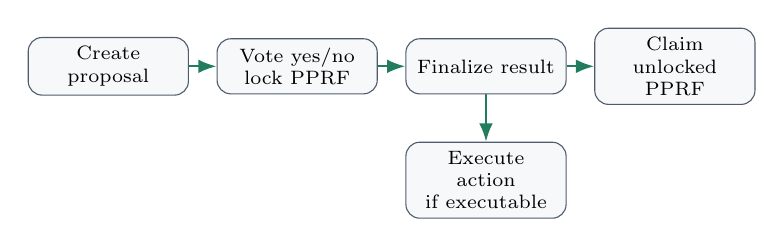
\begin{tikzpicture}[
    flowstep/.style={draw=paperLine, rounded corners=5pt, fill=paperSoft, minimum height=0.7cm, align=center, font=\scriptsize, text width=1.8cm},
    arrow/.style={-Latex, thick, draw=paperGreen},
    node distance=0.35cm
]
    \node[flowstep] (create) {Create proposal};
    \node[flowstep, right=of create] (vote) {Vote yes/no\\lock PPRF};
    \node[flowstep, right=of vote] (finalize) {Finalize result};
    \node[flowstep, below=0.6cm of finalize] (execute) {Execute action\\if executable};
    \node[flowstep, right= of finalize] (claim) {Claim unlocked\\PPRF};
    \draw[arrow] (create) -- (vote);
    \draw[arrow] (vote) -- (finalize);
    \draw[arrow] (finalize) -- (execute);
    \draw[arrow] (finalize) -- (claim);
\end{tikzpicture}
\end{document}
